\documentclass{assignment}
\ProjectInfos{在生活中感知材料的魅力}{GENS1004}{2020-2021学年第一学期}{第三次作业}{固体材料表面的爱与憎——超疏水和超亲水}{陈稼霖}{45875852}
\begin{document}
\begin{ti}
    表征材料的亲水和疏水特性的参数是什么?利用材料的超亲水和超疏水特性分别是如何实现物体的表面清洁的?
\end{ti}
\begin{da}
    表征材料的亲水和疏水特性的参数是表面接触角,即液体/气体截面接触固体表面而形成的夹角。其中表面接触角又分为表面稳定接触角(即固体表面水平状态下的表面接触角)和表面滚动接触角(即固体表面倾角恰好能使液体在其上滚动状态下的表面接触角)。其中,表面稳定接触角大于$150^{\circ}$且滚动接触角小于$10^{\circ}$的情况被定义为超疏水,表面稳定角小于$5^{\circ}$的情况被定义为超亲水。

    使用超亲水材料作为物体表面,当用水冲洗物体表面时,水在物体表面并非呈水滴状聚集,而是在物体表面铺展开从而将物体表面与污物分离开,污物顺水流被冲刷走,从而实现物体表面的清洁。

    使用超疏水材料作为物体表面,则含有污染物的溶液将很难吸附在物体表面,且当用水冲洗物体表面时,水珠迅速从物体表面滚落并带走物体表面的污物,从而实现物体表面的清洁。
\end{da}

\begin{ti}
    气垫层是自然界中生物和动物形成超疏水的重要原因,请进行具体描述和说明。
\end{ti}
\begin{da}
    1805年,托马斯·杨最早提出了光滑表面上的接触角公式(图\ref{Contact-angle-microstates}左):
    \begin{align}
        \cos\theta=\frac{\gamma_{\text{SG}}-\gamma_{\text{SL}}}{\gamma_{\text{LG}}},
    \end{align}
    其中$\gamma_{SG}$为固体和气体之间的表面张力,$\gamma_{\text{SL}}$为固体和液体之间的表面张力,$\gamma_{\text{LG}}$为液体和气体之间的表面张力。Wenzel提出,当固体表面存在凹凸状的微结构,且液体与固体表面微结构的凹凸面直接接触(图\ref{Contact-angle-microstates}中),则此时接触角变为$\theta_W$:
    \begin{align}
        \cos\theta_W=r\cos\theta.
    \end{align}
    其中$r$为凹凸面的实际面积与投影面积的比例,它表征了固体表面的粗糙程度。Cassie与Baxter提出,当固体表面存在凹凸状的微结构,且液体仅与固体表面微结构的凸面接触,即液体悬浮在微结构的表面,在液体和固体之间存在气垫(图\ref{Contact-angle-microstates}右),此时接触角变为$\theta_C$
    \begin{align}
        \cos\theta_C=\varphi\cos\theta-(1-\varphi),
    \end{align}
    其中$\varphi$为固体与液体接触面积占当地固体表面凹凸面实际面积的比例。从上述公式中可以看出,在固、液、气材料相同的情况下,当存在气垫,也即Cassie-Baxter状态下,接触角最大,即疏水性最强。
    \begin{figure}[H]
        \centering
        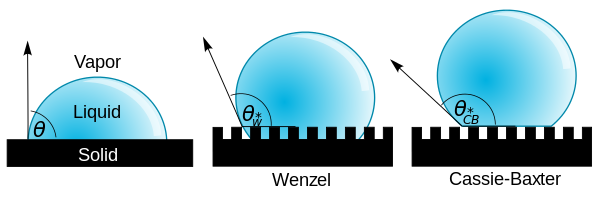
\includegraphics[width=.5\columnwidth]{Contact-angle-microstates.png}
        \caption{各种情况下接触角形成机制的微观结构图。气体环绕的光滑固体表面形成接触角$\theta$;若固体表面存在凹凸状的微结构且液体与固体表面微结构的凹凸面直接接触,则此液滴处于Wenzel状态;若固体表面存在凹凸状的微结构且液体仅与微结构的凸面接触,则此液滴处于Cassie-Baxter状态。}
        \label{Contact-angle-microstates}
    \end{figure}

    各种生物就是通过表面的凹凸状的微结构和液体接触时形成的气垫形成超疏水的。如图\ref{Super-hydrophobic},例如,蝴蝶翅膀表面具有鳞片状的微结构,当水滴落在蝴蝶翅膀上时,会与鳞片间的缝隙之间气垫,因此蝴蝶翅膀表面具有超疏水的特性,使得蝴蝶在雨天仍然可以在空中飞翔;又如,水黾的脚上具有许多密集的油质刚毛,与水接触时形成了很多气垫,这些气垫一方面赋予了水黾的脚以超疏水的性质,另一方面气垫中的空气为水黾提供了额外的浮力,因此水黾可以悬浮在水面上运动而不沉入水底;再如,荷叶表面存在许多微米级的凸起,这些凸起上又有许多纳米级的微粒,当水接触荷叶表面时就可以形成气垫,因此荷叶表面具有超疏水的性质,水珠可以在荷叶表面自由的滚动脱落,减轻了下雨时荷叶支撑的压力。
    \begin{figure}[H]
        \centering
        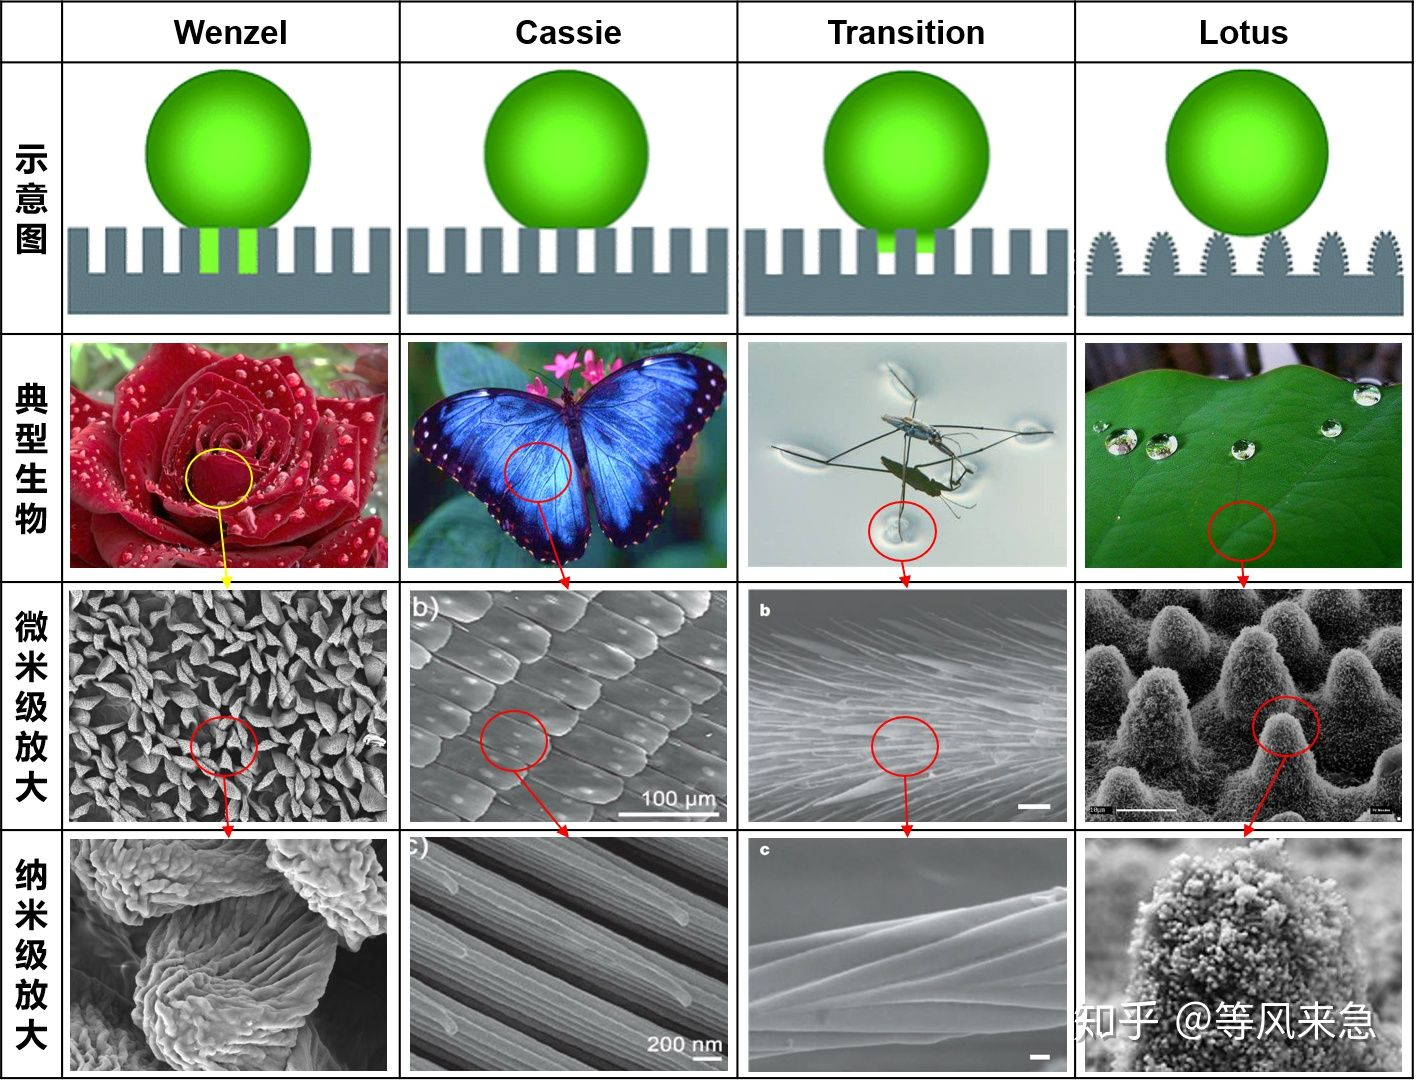
\includegraphics[width=.5\columnwidth]{Super-hydrophobic.jpg}
        \caption{各种生物表面的超疏水结构}
        \label{Super-hydrophobic}
    \end{figure}
\end{da}
\end{document}